\documentclass[12pt]{article}
\usepackage[utf8]{inputenc}
\usepackage{amsmath}
\usepackage{bm}
\usepackage{graphicx}
\usepackage{pdfpages}
\usepackage{hyperref}
\graphicspath { {./images/} }
\title{2DV513 Assignment 2}
\author{Jacob Skoog \\ js224wv}
\begin{document}

\begin{titlepage}
\maketitle
\end{titlepage}

\section {Relational Algebra}\label{sec:relational-algebra}

\subsection {Names of students in 1dv513}\label{subsec:names-of-students-in-1dv513}
\begin {math}
ids = \Pi\_{id}(\sigma\_{code=1dv513}(enrolled))
\end {math}
\\
\begin {math}
answer = \Pi\_{name}(\sigma\_{id \in ids}(student))
\end {math}

\subsection {Names of students in both 1dv513 and 2dv513}\label{subsec:names-of-students-in-both-1dv513-and-2dv513}
\begin {math}
ids1dv513 = \Pi\_{id}(\sigma\_{code=1dv513}(enrolled))
\end {math}
\\
\begin {math}
ids2dv513 = \Pi\_{id}(\sigma\_{code=1dv513}(enrolled))
\end {math}
\\
\begin {math}
union = ids1dv513 \cup ids2dv513
\end {math}
\\
\begin {math}
intersection = ids1dv513 \cap ids2dv513
\end {math}

\paragraph{If} interpreted as a union of students in 1dv513 and 2dv513:
\begin {equation}
\Pi_{name}(\sigma_{id \in union}(student))\label{eq:equation1}
\end {equation}

\paragraph{If} interpreted as an intersection of students in both 1dv513 and 2dv513:
\begin {equation}
\Pi_{name}(\sigma_{id \in intersection}(student))\label{eq:equation2}
\end {equation}

\subsection {Who teaches 2dv610}\label{subsec:who-teaches-2dv610}
\begin{math}
\Pi\_{lecturer} (\sigma\_{code=2dv610}(subject))
\end{math}

\subsection {Who teaches 1dv513 and 2dv513}\label{subsec:who-teaches-1dv513-and-2dv513}

\paragraph{If} interpreted as unions of teachers of both 1dv513 and 2dv513:
\begin {equation}
\Pi_{lecturer} (\sigma_{code=1dv513}(subject) \cup \sigma_{code=2dv513}(subject))\label{eq:equation3}
\end {equation}
\paragraph{If} interpreted as the intersection of those teaching in both 1dv513 and 2dv513:
\begin {equation}
\Pi_{lecturer} (\sigma_{code=1dv513}(subject) \cap \sigma_{code=2dv513}(subject))\label{eq:equation4}
\end {equation}

\subsection {Names of students *not* taught by Ilir}\label{subsec:names-of-students-*not*-taught-by-ilir}

\begin {math}
codes = \Pi\_{code}(\sigma\_{lecturer=Ilir}(subject))
\end{math}
\\
\begin {math}
IlirStudents = \Pi\_{id}(\sigma\_{code \in codes}(enrolled))
\end {math}
\\
\begin {math}
answer = \Pi\_{name}(\sigma\_{id \notin IlirStudents}(student))
\end {math}

\section {FDs and Normalisation}\label{sec:fds-and-normalisation}
\subsection {Functional Dependencies}\label{subsec:functional-dependencies}

\begin {figure}[h]
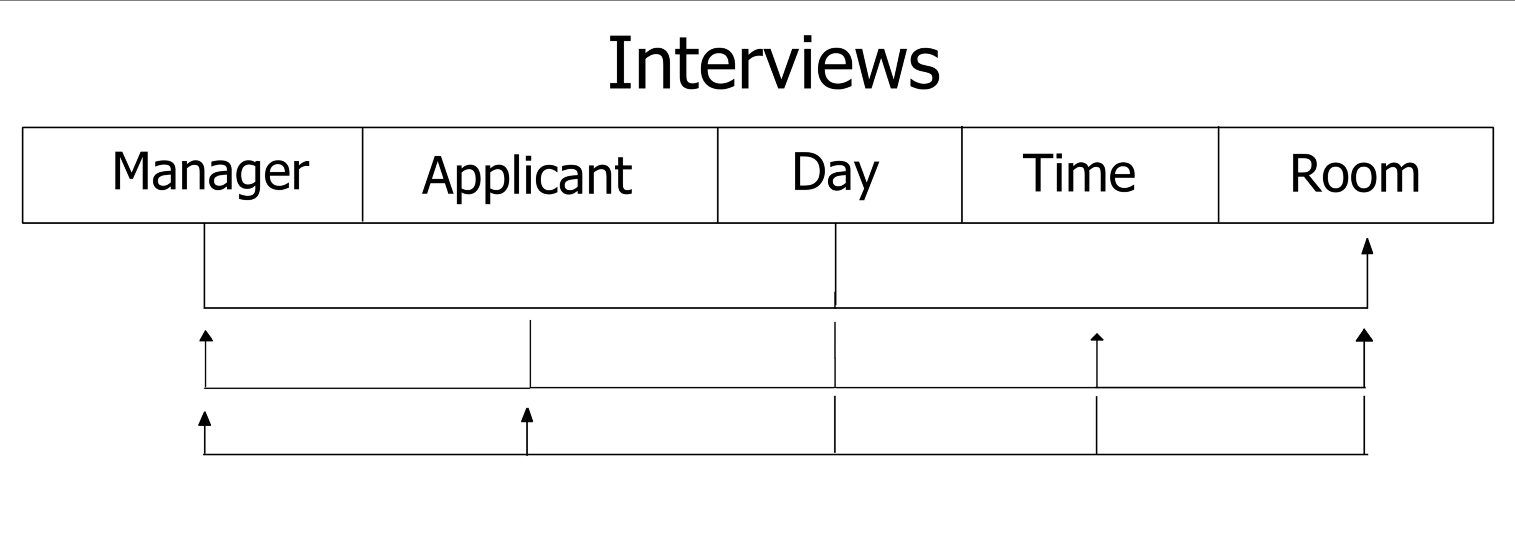
\includegraphics [width=\textwidth]{FD}
\caption { The functional dependencies of the Interviews Relation	}
\label{fig:fd1}
\end {figure}

As can be seen in figure~\ref{fig:fd1}, three functional dependencies have been identified.

\subsubsection {\(\{Manager, Day\} \mapsto \{Room\}\)}
Since a manager is only in a single room in any set day, you can determine the room from the Manager and Day attributes.

\subsubsection {\(\{Applicant, Day\} \mapsto \{Manager, Time, Room\}\)}
As an applicant will only have a single interview in a set day, and a single interview will have a single manager, at a single time, at a single room, this dependency holds.

\subsubsection {\(\{Day, Time, Room\} \mapsto \{Manager, Applicant\}\)}
If day, time, and room are known they will identify a unique interview, which will have a single manager and applicant.

\subsection {The keys of the relation}\label{subsec:the-keys-of-the-relation}

\subsubsection {Candidate Keys}

Since \(\{Applicant, Day\} \mapsto \{Manager, Time, Room\}\) (1) and \(\{Day, Time, Room\} \mapsto \{Manager, Applicant\}\) (2) will both identify a single unique tuple in R, they are candidate keys. \\
As the choice of primary key is arbitrary at this point, I will choose (1) as the primary key and (2) as the secondary key.

\subsection {3NF but not BCNF}\label{subsec:3nf-but-not-bcnf}
\subsubsection {1NF}

All the values are atomic, so the relation is 1NF\@.

\subsubsection {2NF}

The only non-prime attribute is 'Manager'.

The relation is 2NF as Manager is functionally dependent on the chosen primary key (and the secondary key).
The functional dependency is furthermore full, as the removal of any attribute would break the functional dependency.
The same is also true of the secondary key.

\subsubsection {3NF}

As stated when discussing 2NF, the only non-prime attribute is 'Manager', and Manager is not functionally dependent on any other non-prime attribute, as there is no other non-prime attribute.
Or, to use the general definition of 3NF:\\
There are three non-trivial functional dependencies in the relation.
Two of these are superkeys of the relation (fulfilling clause (a) of the general definition).
The only FD \(X \mapsto A\) where X is not a superkey is the FD \(\{Manager, Day\} \mapsto \{Room\}\), and here A is a prime attribute \{Room\}, thus fulfilling clause (b).
\\Thus, the relation is 3NF\@.

\subsubsection {BCNF}
As mentioned above, one of the functional dependencies fulfilled clause (b) of 3NF, but that clause is not allowed in BCNF. The relation is therefore not in BCNF\@.

\subsection {Decompose into BCNF}\label{subsec:decompose-into-bcnf}

The decomposition must pass the non-additive join test.
I propose the following decomposition: \(R_1(Manager, Day, Room), R_2(Manager, Applicant, Day, Time)\)\\
Then, \(R_1 \cap R_2 = \{Manager, Day\}, R_1 - R_2 = \{Room\}, and \{Manager, Day\} \mapsto \{Room\} \in F^+\), thus this decomposition passes the test.

\begin {figure}[h]
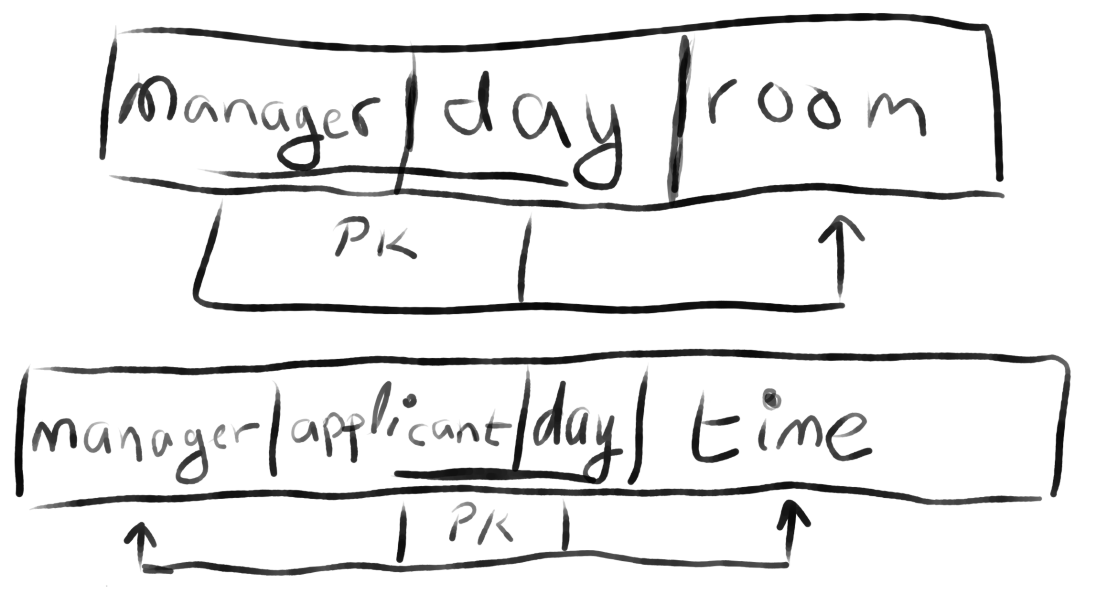
\includegraphics[width=\textwidth]{BCNF}
\caption{The two decomposed relations and their functional dependencies}\label{fig:ER}
\end {figure}

As can be seen on the diagram~\ref{fig:ER}, the two relations are now BCNF-compliant, as now whenever an FD \(X \mapsto A\) holds, X is a superkey (as neither of the keys above can lose any attribute).

\subsection {ER Diagram}\label{subsec:er-diagram}
\begin {figure}[h]
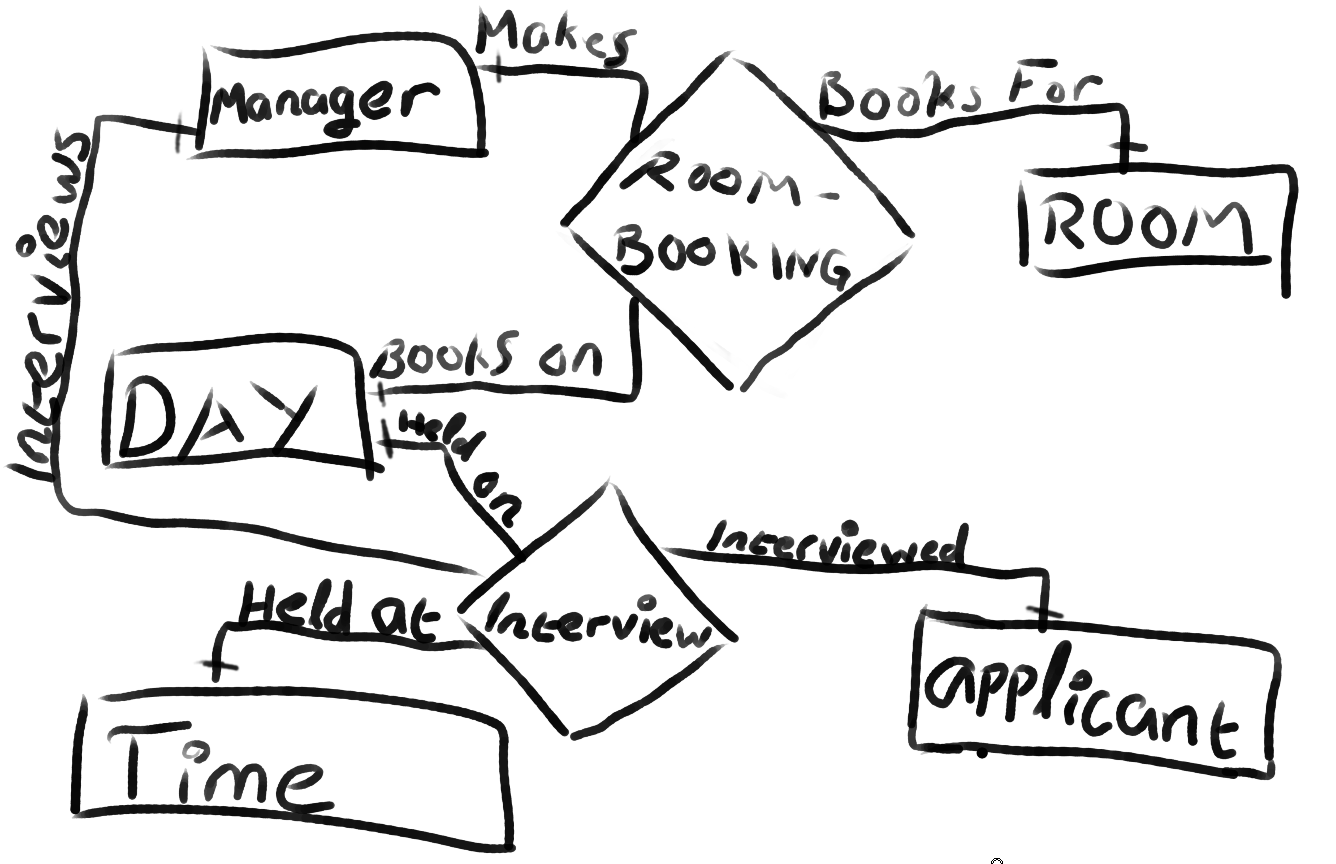
\includegraphics[width=\textwidth]{ER}
\caption {Entity Relation Diagram for the Relation}\label{fig:figure2}
\end {figure}

\section {Setting up the reddit database}\label{sec:setting-up-the-reddit-database}

See the following pages for ER diagram and schemas with types.
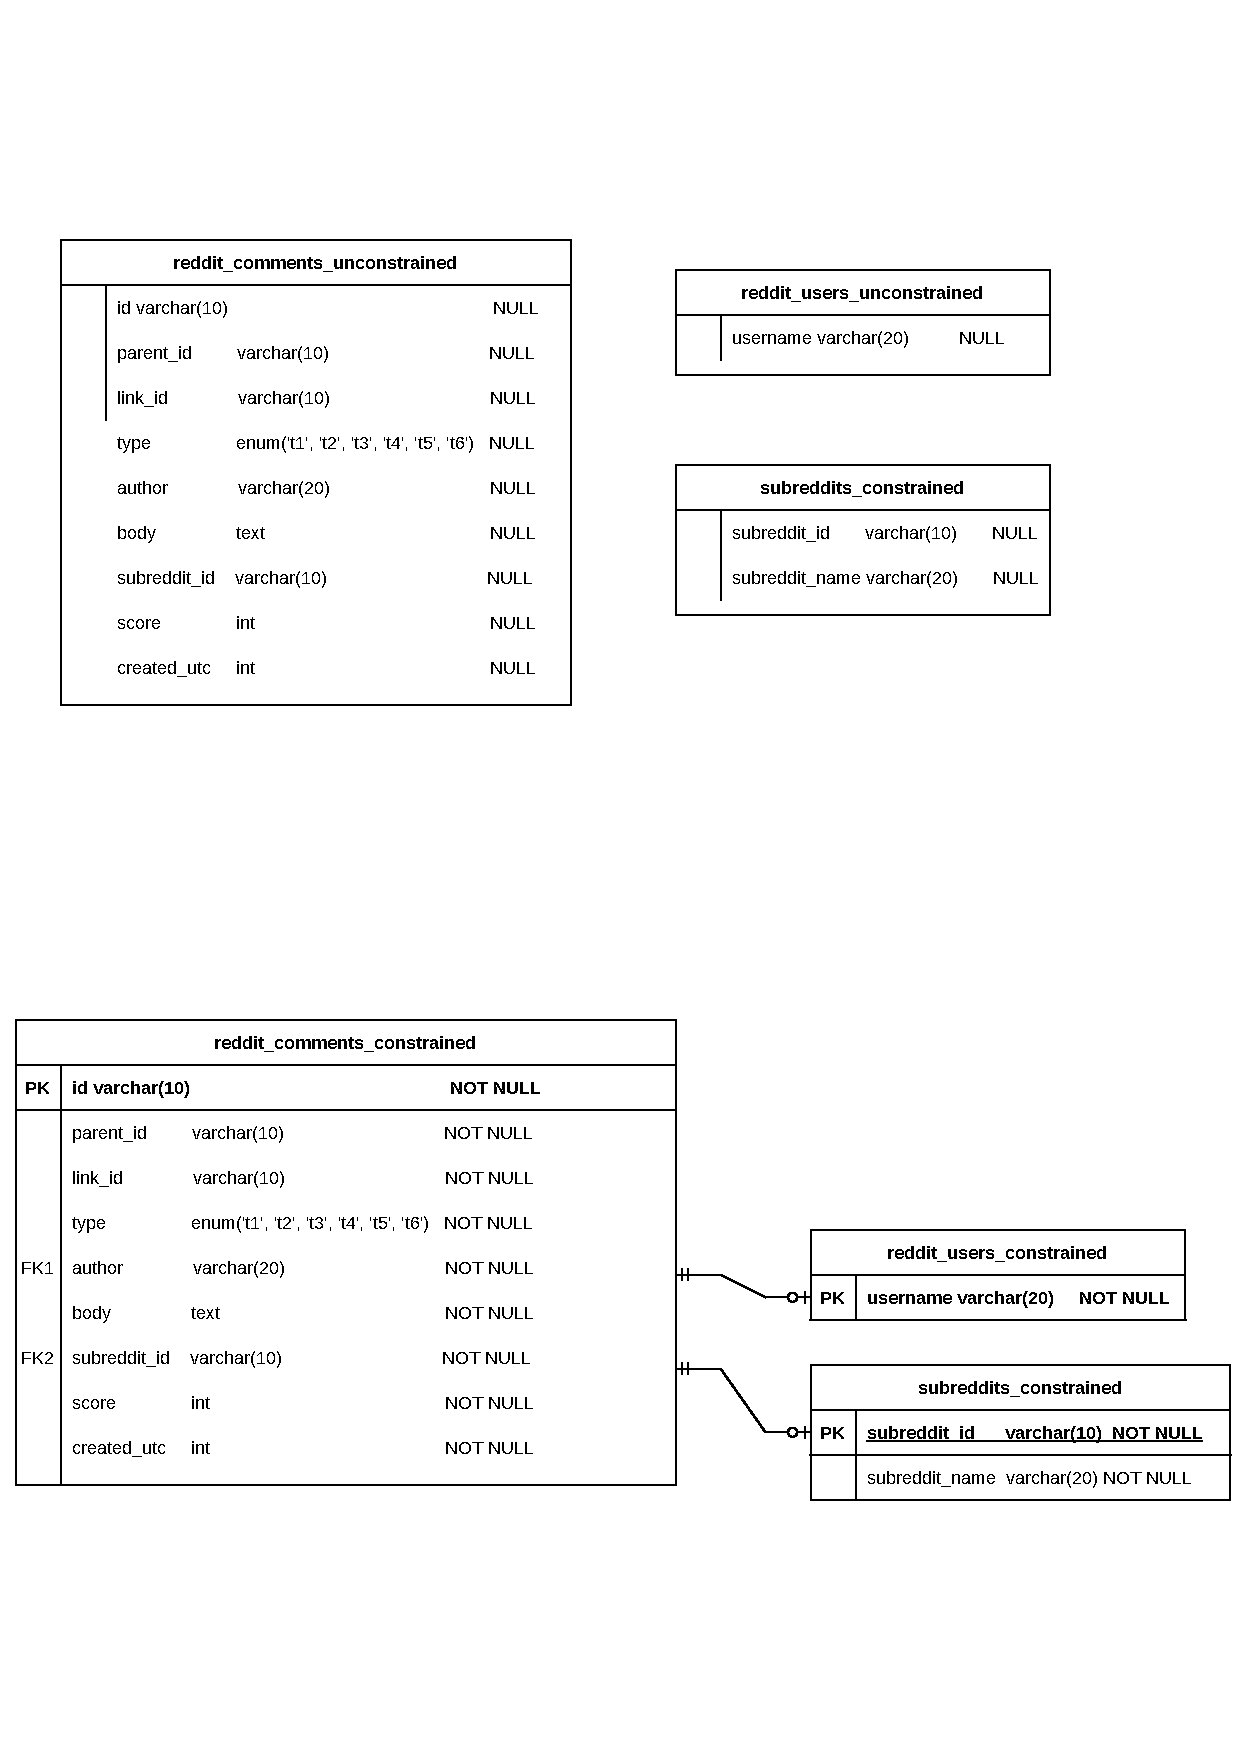
\includepdf[pages=-]{DB_Schemas.pdf}
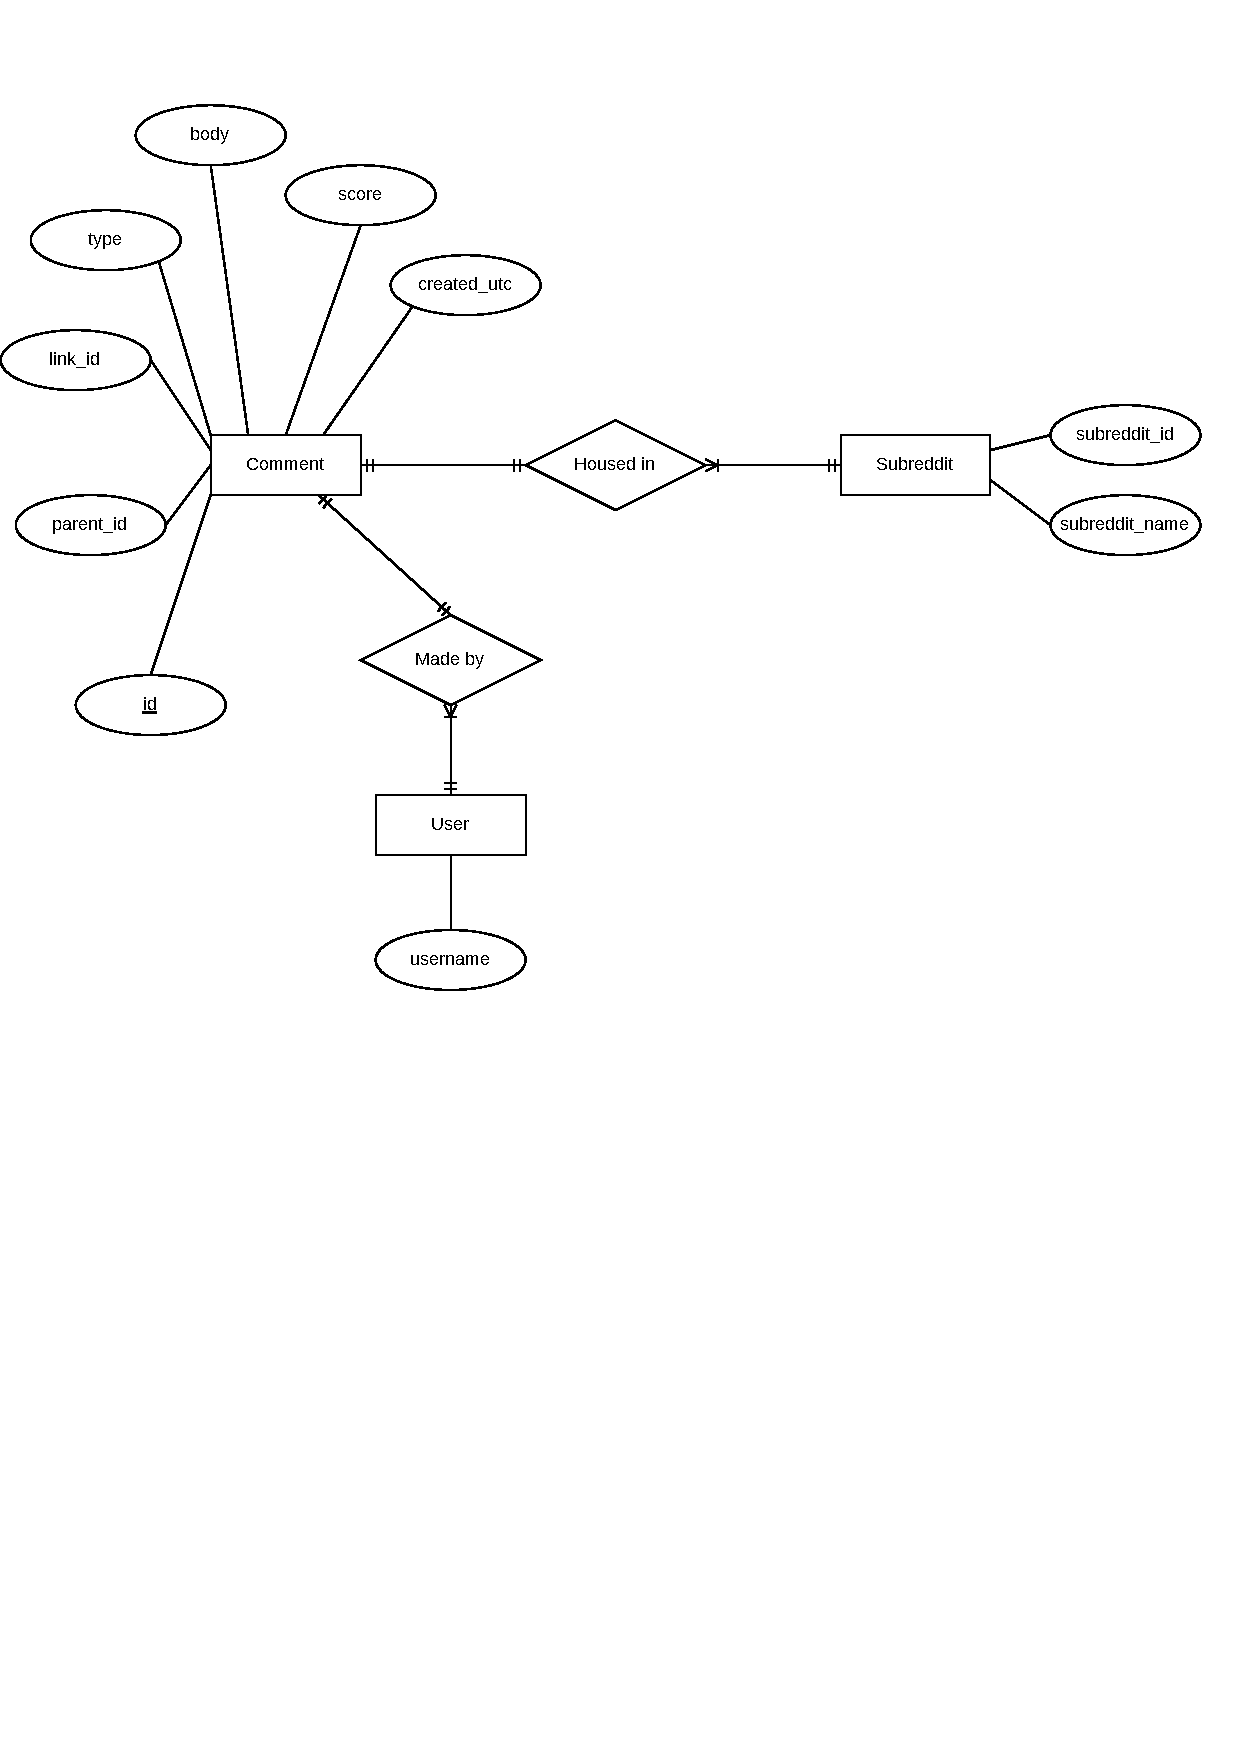
\includepdf[pages=-]{Reddit_DB_ER.pdf}

\section {Importing the data}\label{sec:importing-the-data}
Link to repo: \url{https://github.com/SkoogJacob/RedditDB}

See the following page for test results.
I used three different tests to load the data.
All tests were run in Java using a JDBC driver.
Loading of the unconstrained tables was done using multithreading, with each thread handling batches of 2000 records.

Loading the constrained tables was done on a single thread in batches of 15000 entries.

The test staging entries first to the unconstrained tables works just like the first test.
The only difference is that once the unconstrained tables are loaded it queries the SQL database to load all entries over to the constrained tables, trusting the SQL database to handle batching and multithreading.

The first tests, labelled "unconstrained" inserted the data into a table without any constraints.
This was the fastest to run, taking about 1.5 seconds on average to add all the entries.
This design does have the drawback of having an immense amount of duplicate records in the Redditor and Subreddit tables.

The second group of tests, labelled "constrained" was by far the slowest.
This is, in large part I believe, due to the code adding entries needing to check the database to avoid adding duplicate entries in the batches.
The execution speed would be even worse if the SQL server was run on a separate machine and all of these queries to avoid duplicates had to wait for network latency.
In addition, I was unable to use multithreading when adding entries to the heavily constrained table.

The last set of tests, labelled "test using staging to unconstrained tables" was much faster than the constrained tests, but it ends up with the same end results.
It does so by first adding all entries to the unconstrained tables as in the first round of tests.
It then queries SQL and asks it to add all distinct entries to the corresponding constrained table.

This test was run on the small file (90MB) which contains around 150--000 entries.

This last method will be the one I use to load in the actual database for the next part of the report.
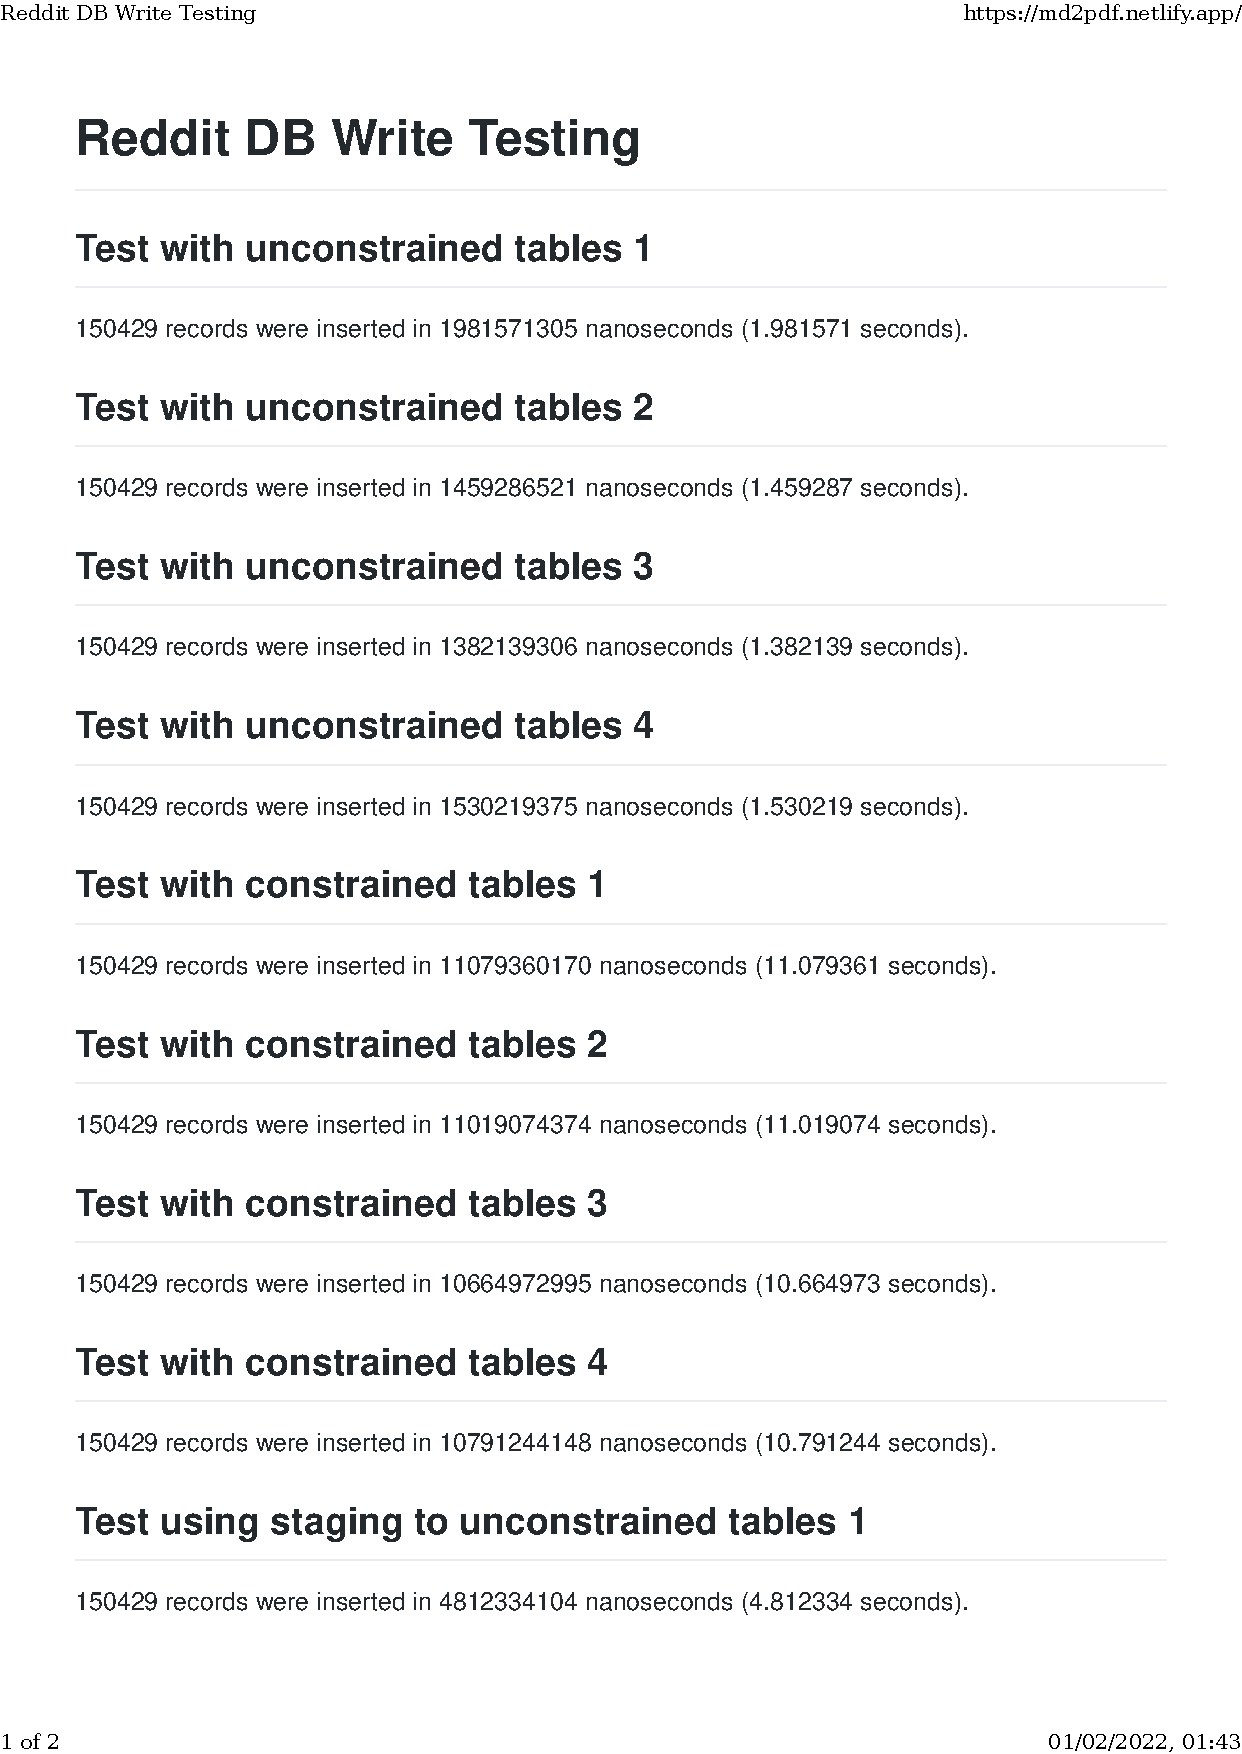
\includepdf[width=\textwidth, pages=-]{results.pdf}

After running this test I did some changes to the code and tried with adding most indexes and such after inserting the data into the table.
I did this because after inserting the entries from the 2012--12 file my database program was unable to drop the table if the indexes were still on it.
So I ended up modifying the loader code for the constrained table to insert with the bare minimum indexes active (only primary key and foreign keys).
I was also able to improve the code significantly and removed the need to query the database to avoid inserting duplicates into the redditor and
subreddits tables.
I was still unable to use multithreading, however, as it still led to conflicting locks (it added exactly 150--000 entries on the testing dataset, losing about 400 entries).

When trying to load the larger datasets I discovered that the code I used for staging was entirely broken for large datasets.
This is because the method I used required the entire source table being locked while it read from it.
But InnoDB has a default cap of around 6 million locked rows, so the 15GB dataset blew right past that.
To use the pre-staging test I would have to rewrite it to work in smaller batches.

The reason I will not implement this, though, is that after these improvements to loading the constrained table directly the staging table is no longer faster.
This is likely because the staging loader is simply doing more work than the constrained loader.
On the database side it is first doing the unconstrained loader and then the constrained loader afterwards, and the testing times are fairly consistent with this hypothesis.
Before the constrained loader had a huge inefficiency in that it was constantly querying the database to avoid inserting duplicates, so loading through a staging table ended up being faster just on virtue of not doing these redundant checks.
Now that that huge inefficiency is amended, there is no longer any advantage to using staging, at least not in the way that I implemented it.
Due to this I will simply abandon it and stick to my constrained loader.

I also significantly increased batch size for both the unconstrained and constrained loaders, as each comment having maximum body length was incredibly unlikely.
The batch sizes were increased to 6000 entries per batch for the unconstrained loader and 50--000 for the constrained loader.

The following two pages will have the results from loading the smaller test set as well as loading the large 2012--12 file.

\subsection{Conclusions}\label{subsec:loading_conclusions}

So, in total, adding the data first and then adding in the constraints afterwards seemed to offer the best performance when performing a large sequence of
operations.
This is because when the database has all the data loaded already, it can organize its work of indexing the data effectively.
When the indexes are already in place it is constantly re-ordering the table to abide by the index rules, and this constant reordering is quite expensive.

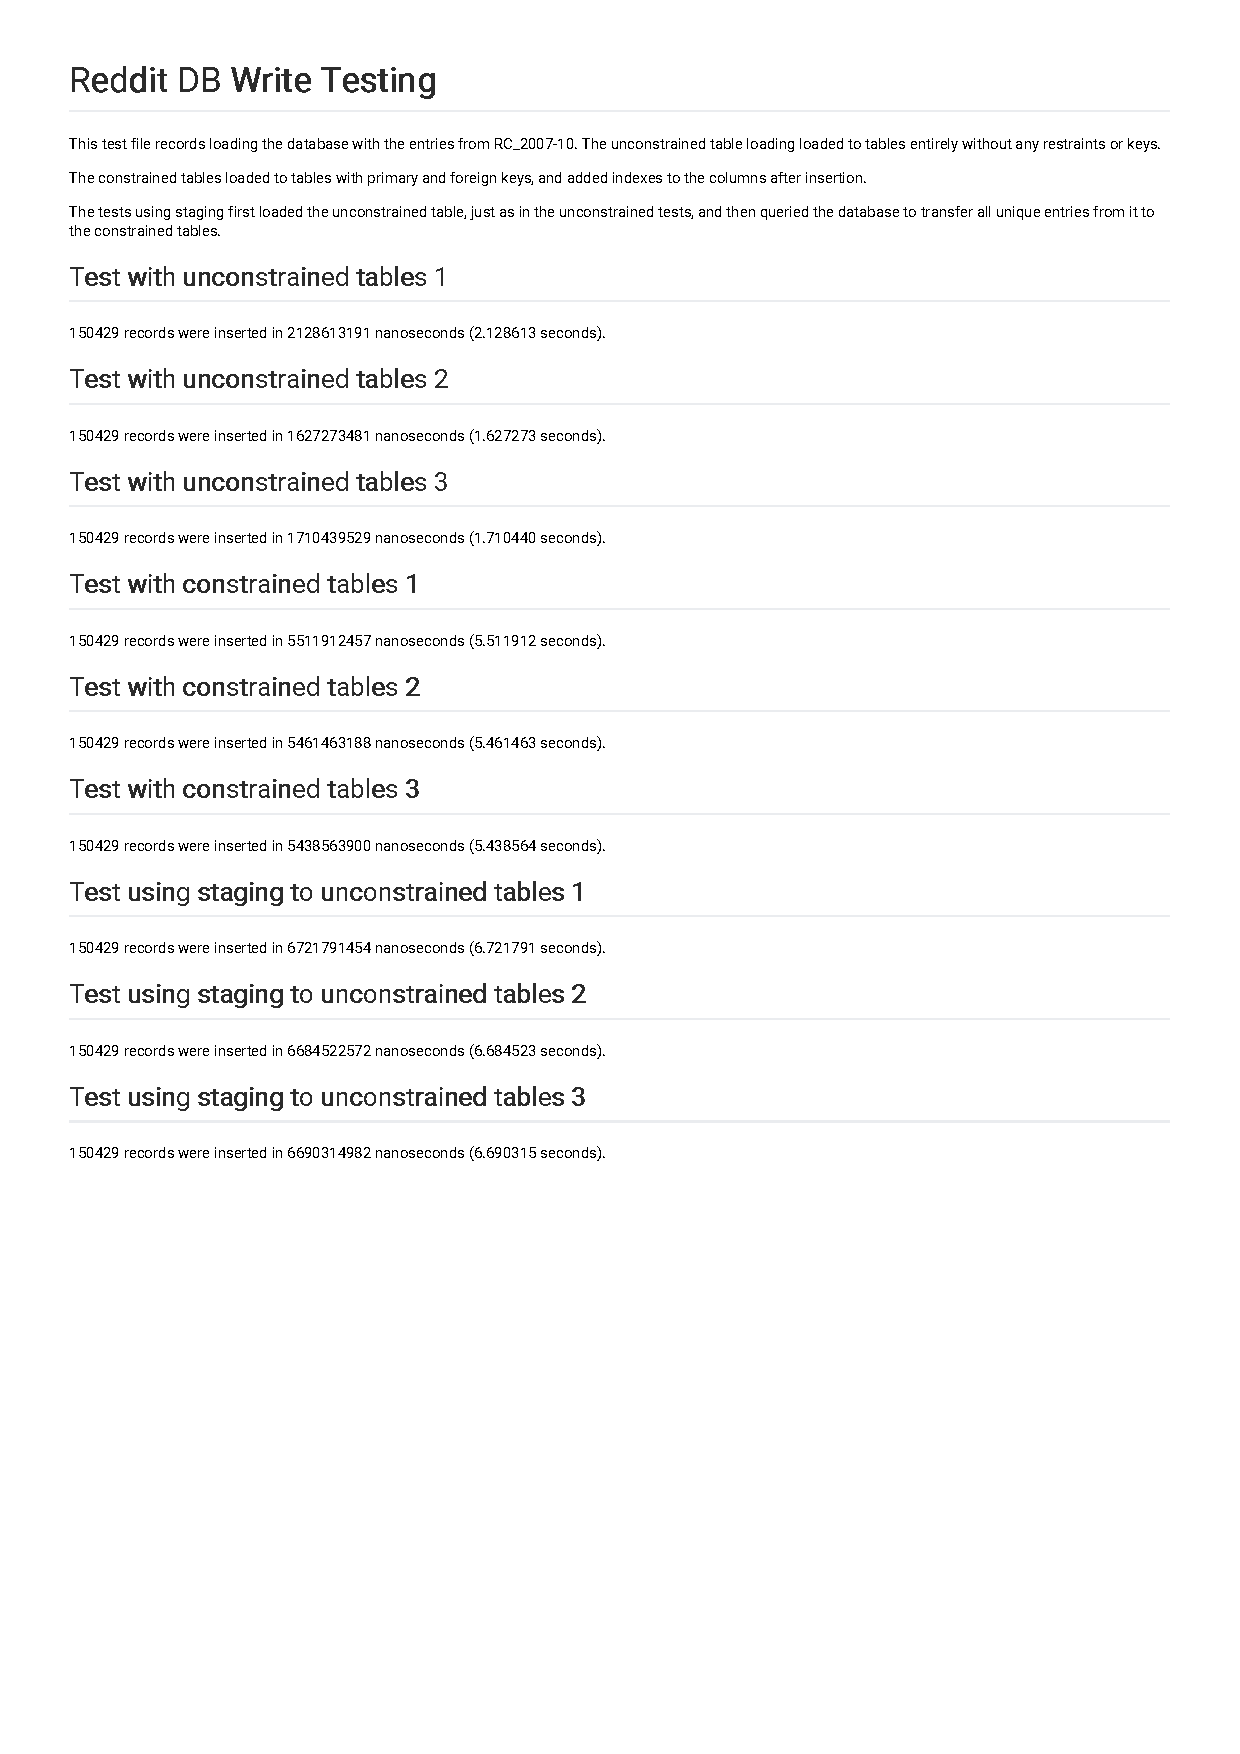
\includepdf[width=\textwidth, pages=-]{report_improved.pdf}
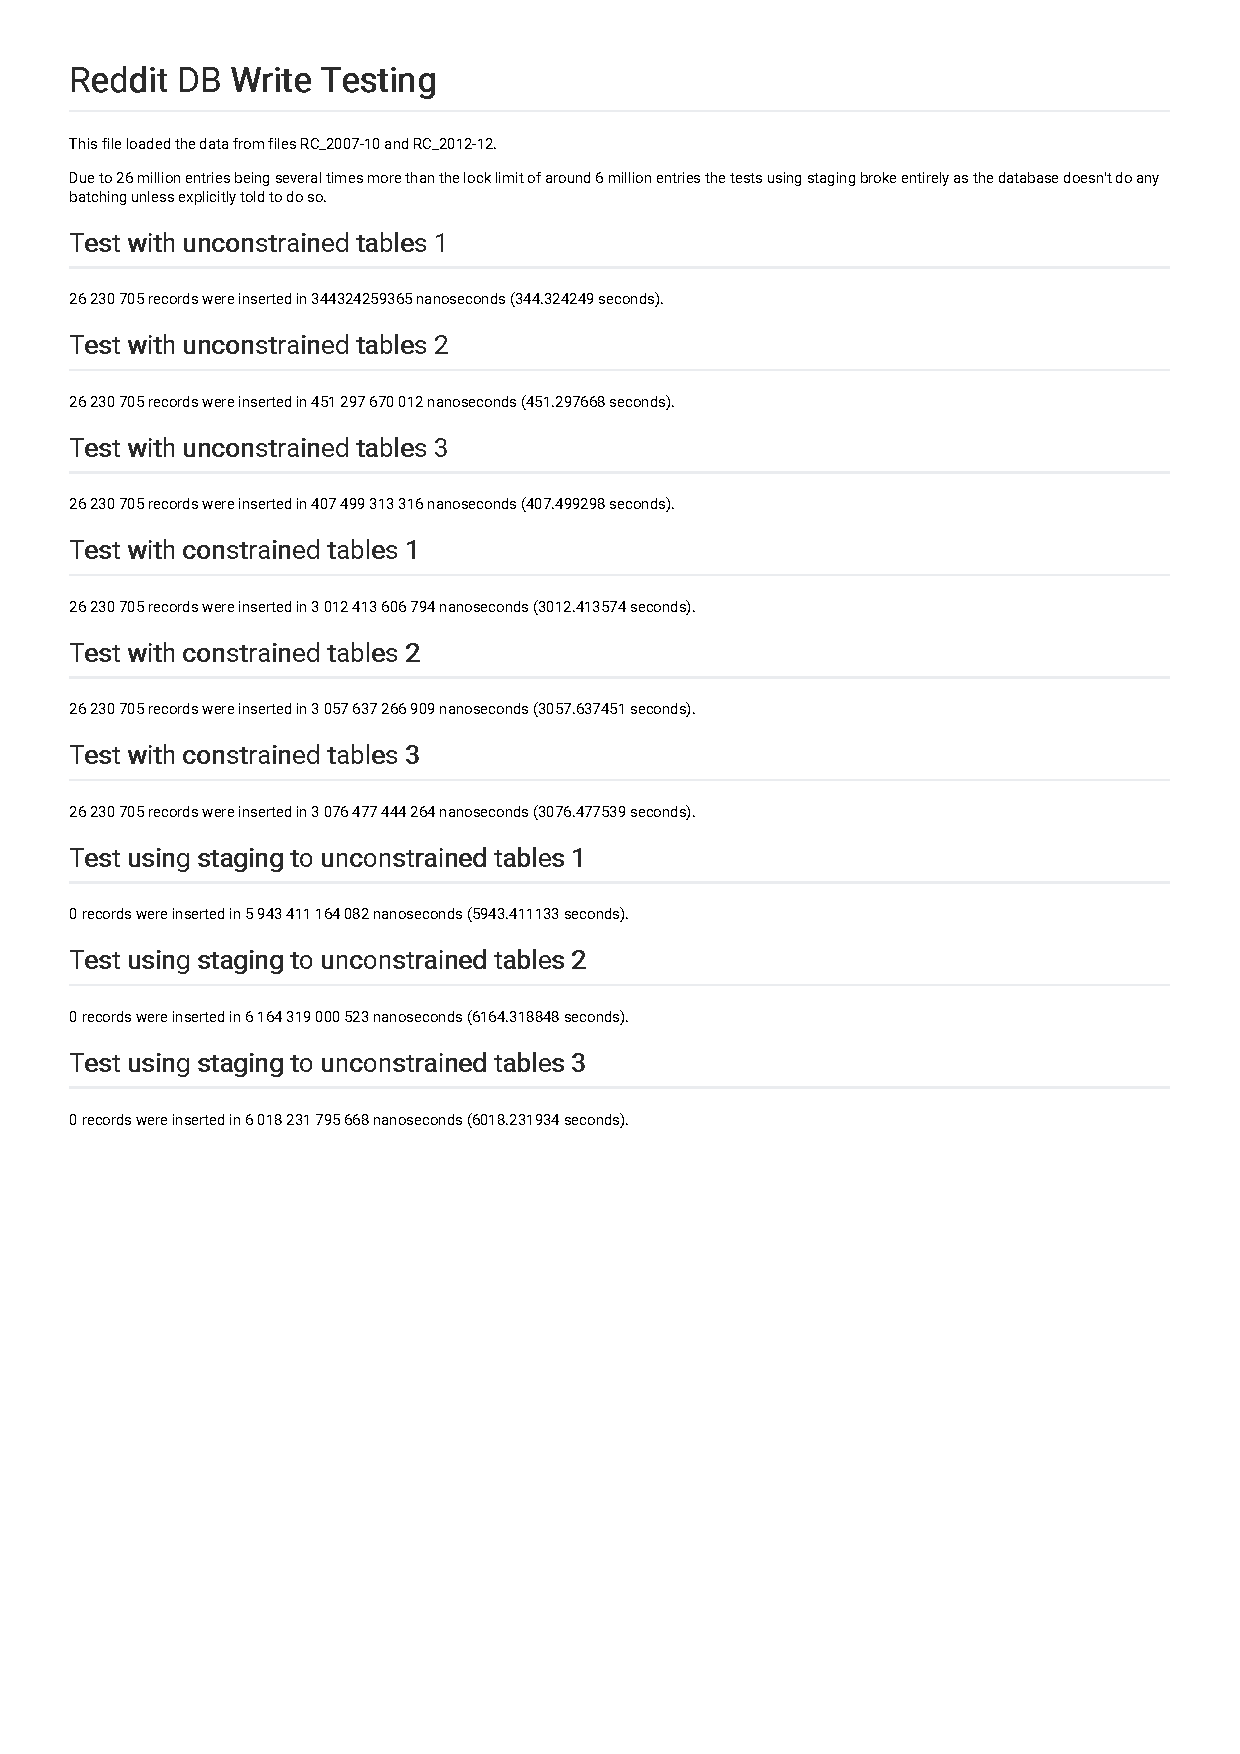
\includepdf[width=\textwidth, pages=-]{report_improved_big_data.pdf}

\section {SQL Queries}\label{sec:sql-queries}
\subsection {Number of comments by a specific user}\label{subsec:comments-by-user}
    \begin{verbatim}
        SELECT COUNT(*)
          FROM   schema.comments_constrained
          WHERE  author='username';
    \end{verbatim}
    All usernames can be queried from the schema.redditors table.

\subsection{Comments per day in subreddit}\label{subsec:comments-per-day}
    First, I define a SQL function to translate the subreddit\_id to subreddit\_name for prettier presentation.
    I also define basically the same function but in the other direction if it should be needed.

    \begin{verbatim}
CREATE FUNCTION
    get_subreddit_name(parameter_subreddit_id VARCHAR(10))
    RETURNS VARCHAR(20)
    READS SQL DATA
    BEGIN
        RETURN
            (SELECT subreddit_name
            FROM schema.subreddits_constrained
            WHERE subreddit_id = parameter_subreddit_id);
    END;
    \end{verbatim}
    A function to translate epoch time to Dates is also defined.
    \begin{verbatim}
CREATE FUNCTION
    epoch_to_date(parameter_epoch INT)
    RETURNS INT
    READS SQL DATA
    BEGIN
        RETURN (DATE(FROM_UNIXTIME(parameter_epoch)));
    END;
    \end{verbatim}
    To simplify getting the desired data I also create a view in the database using the queries below.
    \begin{verbatim}
CREATE VIEW schema.comment_date_view AS
    SELECT
        id,
        get_subreddit_name(schema.comments_constrained.subreddit_id)
            AS subreddit_name,
        epoch_to_date(schema.comments_constrained.created_utc)
            AS posted_date
    FROM schema.comments_constrained;
    \end{verbatim}

    With this in place, I define a stored procedure:
    \begin{verbatim}
CREATE PROCEDURE posts_per_day (
    IN p_subreddit_name VARCHAR(20),
    OUT p_posts_per_day FLOAT
)
    READS SQL DATA
    BEGIN
        SET p_posts_per_day =
            (SELECT AVG(posts_in_day) AS avg_per_day FROM (
            SELECT
                COUNT(posted_date) AS posts_in_day
            FROM test_db.comment_date_view
            WHERE subreddit_name = p_subreddit_name
            GROUP BY posted_date)
        AS posts_per_day);
    END;
    \end{verbatim}

    Calling this procedure as below will then give average posts per day for the passed subreddit name.
    \begin{verbatim}
CALL posts_per_day ('subreddit_name', @out);
SELECT @`out`;
    \end{verbatim}

\subsection{How many comments include the word 'lol'}\label{subsec:how-many-comments-include}

Start by defining a procedure that stores the number of comments with the desired word in the out parameter.

\begin{verbatim}
CREATE PROCEDURE posts_containing (
    IN p_term VARCHAR(50),
    OUT number_containing INT
)
    READS SQL DATA
    BEGIN
        SET number_containing = (SELECT COUNT(*) FROM
            (SELECT * FROM test_db.comments_constrained
            WHERE body LIKE CONCAT('%', p_term, '%')) as contains_term);
    END;
\end{verbatim}

    Then it can easily be called as
    \begin{verbatim}
CALL posts_containing ('lol', @ccc);
SELECT @`ccc`;
    \end{verbatim}

    Whether the method should demand spaces around the search phrase is debatable.
    In the case of lol, the word is oftentimes used as one part of a longer word, so it would miss some counts there.
    On the other hand, it is likely also including some entries that wouldn't fit what the user of the procedure likely intended.

    Due to this, I think letting the caller of the method put in whitespaces themselves if they want stricter results is appropriate, and I will leave it as is.

    \subsection{Commenters of thread T have participated in what subreddits?}\label{subsec:what-subreddits}

    In MariaDB it is not possible to return multiple values from stored procedures or functions, so the stored procedure cannot return the results it found for further processing.

    \begin{verbatim}
CREATE PROCEDURE subreddits_from_link_id (
    IN p_link_id VARCHAR(10)
)
    READS SQL DATA
    BEGIN
        SELECT DISTINCT get_subreddit_name(subreddit_id) AS subreddit
         FROM test_db.comments_constrained
         WHERE author IN
               (SELECT DISTINCT author
                FROM test_db.comments_constrained
                WHERE link_id = p_link_id
                AND NOT author='[deleted]'
                );
    END;
    \end{verbatim}

    \subsection{Which users have the highest and lowest scores?} \label{subsec:user-high-low-scores}

    These two question are basically the same, the only difference is if it is ORDER BY \ldots ASC or ORDER BY \ldots DESC .
    I will show the DESC variant below.

    \begin{verbatim}
CREATE PROCEDURE user_highscores (
)
    READS SQL DATA
BEGIN
    SELECT author, SUM(score) AS total_score
        FROM comments_constrained
        WHERE NOT author='[deleted]'
        GROUP BY author
        ORDER BY total_score DESC;
END;
    \end{verbatim}

    \subsection{Which subreddits have highest and lowest scores?} \label{subsec:subreddit-high-low-scores}
    This is basically the same as the previous question about user high scores and lowest scores, but querying for subreddits instead.
    Showing a stored procedure below.

    \begin{verbatim}
CREATE PROCEDURE subreddit_lowscores (
)
    READS SQL DATA
    BEGIN
        SELECT
        get_subreddit_name(subreddit_id) AS subreddit,
        SUM(score) AS total_score
            FROM comments_constrained
            GROUP BY subreddit
            ORDER BY total_score;
    END;
    \end{verbatim}

    \subsection{All users someone might have interacted with} \label{subsec:potential-interactions}

This means getting all links that a user has posted in, getting all comments on those links and selecting distinct authors.

    \begin{verbatim}
CREATE PROCEDURE get_interactions(
    IN p_redditor VARCHAR(20)
)
    READS SQL DATA
    BEGIN
        SELECT DISTINCT author
            FROM test_db.comments_constrained
            WHERE link_id IN
                (
                    SELECT link_id
                    FROM test_db.comments_constrained
                    WHERE author=p_redditor
                 )
            AND author NOT IN ('[deleted]', p_redditor);
    END;
    \end{verbatim}

    \subsection{All users who have only posted in one subreddit} \label{subsec:only-one-subreddit}

    This procedure gets the author and subreddit\_id columns from the comments table, and uses select distinct to
    then be able to count the number of rows grouped by author.
    Then getting those with only one subreddit is as easy as querying for where count=1.

    \begin{verbatim}
CREATE PROCEDURE only_n_subreddits(IN p_n INT)
    READS SQL DATA
    BEGIN
        SELECT *
        FROM (SELECT author, COUNT(*) AS `subreddit_count` FROM
            (SELECT DISTINCT author, subreddit_id
             FROM comments_constrained
             WHERE NOT author='[deleted]')
                AS author_reddits
              GROUP BY author) AS `only_one_reddit`
        WHERE subreddit_count<=p_n;
    END
    \end{verbatim}

\end{document}
